\documentclass[11pt]{article}
\usepackage[margin=2cm]{geometry}
\usepackage{graphicx,amsmath,amssymb,url,color,multirow}

\newcommand{\R}{\mathbb{R}}		% For reals
\newcommand{\prob}[1]{{\textsf{\small #1}}}    % For problem names

\begin{document}
\today

\section{Lockwood}
\label{sec:lockwood}
This is a pump-and-treat groundwater remediation problem from the Lockwood Solvent Groundwater Plume Site located near Billings, Montana.  The basic version considered in \cite{Matott2011} is to determine extraction rates for six wells in order to minimize operating costs, subject to $m=2$ simulation-based constraints on the steady state flux from two different contaminant plumes. Figure~\ref{fig:site} illustrates the LSGPS scenario considered.

\begin{figure}[tb]
\begin{center}
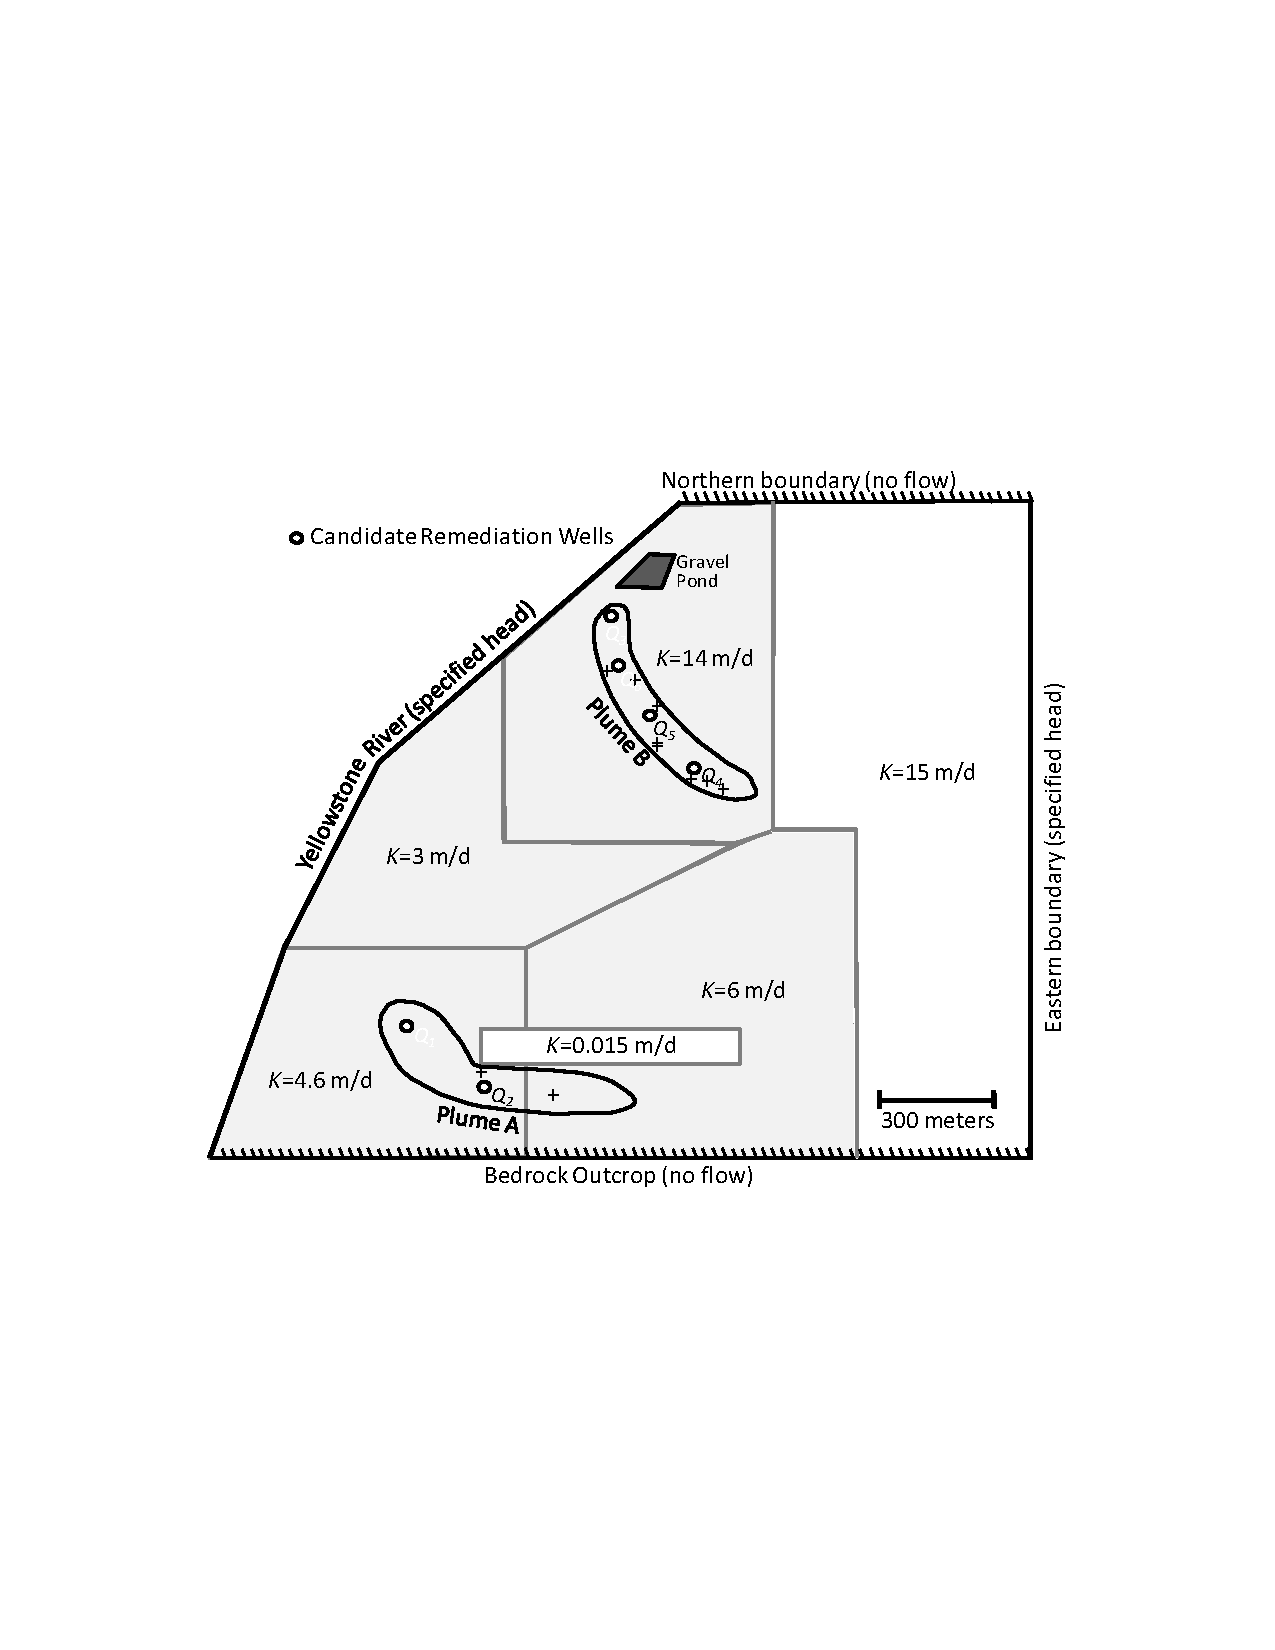
\includegraphics[width=.6\linewidth]{images/Lockwood_Site.pdf}
\end{center}
\caption{The pump and treat site (figure from \cite{Matott2011}).\label{fig:site}}
\end{figure}

A generalization of this problem is to also determine the number of wells and their locations. Mathematically, this general problem can be formulated as
\begin{equation}
\min_{r,x,y,w} \left\{\sum_{i=1}^{w_1} r_i + \sum_{i=3}^{2+w_2} r_i+ 20000(w_1+w_2) : 
 c_1(x,y,r)=0, 
 c_2(x,y,r)=0,
 (r,x,y)\in\mathcal{D}, 
 w \in \mathcal{Z}
 \right\},
 \label{eq:lockwood}
\end{equation}
where $w_i$ corresponds to the number of wells to be installed in a zone containing plume $i$, $(x,y)$ denote the locations of each well, and $r$ denotes the pumping rates. The rates (in feet/day) and locations (in feet) are continuous variables and are restricted to a box $\mathcal{D}$ denoted by simple bound constraints (e.g., $l_i\leq r_i \leq u_i$). The numbers of wells are (unrelaxable) integers with $\mathcal{Z}=\left\{w:w_1\in\{0,\cdots,2\},w_2\in\{0,\cdots,4\}\right\}$.  Table~\ref{tab:lockwood} provides the lower and upper bounds for each parameter. 

The two terms in the objective correspond to the cost of operating the installed wells and the cost of installation, respectively. The two nonlinear constraints, $c_1$ and $c_2$, capture the flux from the two contaminant plumes and depend on the output from the Bluebird simulator \cite{bluebird}. 

From the general formulation in (\ref{eq:lockwood}) we define four different problems:
\begin{description}
 \item[\prob{LOCKWOOD-BASIC}] A 6-dimensional NLP where the locations $(x,y)$ of $w_1+w_2=6$ wells are fixed to belong to
  \[
  \mathcal{W} = 
  \{(2670, 1520), (3340, 1000), (4430, 5020), (5130, 3715), (4770, 4170), (4500, 4585)\},
  \]
  and the pumping rates $r$ are to be determined.
 \item[\prob{LOCKWOOD-PLUS}] A 12-dimensional MINLP where the only possible locations
  of the wells are $\mathcal{W}$. 
  Pumping rates $r$ and a binary vector indicating which of the 6 possible wells should be installed are to be determined.
 \item[\prob{LOCKWOOD-XY}] An 18-dimensional NLP where the number of wells ($w_1=2,w_2=4$) is fixed.
 \item[\prob{LOCKWOOD-XY-PLUS}] A 20-dimensional MINLP where all variables are free.
\end{description}

Initial values for any free variables are provided in Table~\ref{tab:lockwood}.

For optimization solvers that cannot handle blackbox constraints, the penalized, box-constrained problem
\begin{equation}
\min_{r,x,y,w} \left\{\sum_{i=1}^{w_1} r_i + \sum_{i=3}^{2+w_2} r_i+ 20000(w_1+w_2) 
  + 10000\sum_{i=1}^2 |c_i(x,y,r)| :
 (r,x,y)\in\mathcal{D}, 
 w \in \mathcal{Z} \right\}
 \label{eq:lockwoodpenalty}
\end{equation}
is recommended.







\begin{table}
\begin{center}
 \begin{tabular}{|c|c|rr|}
\hline
\textbf{Parameter} & \textbf{Initial} & \textbf{Lower} & \textbf{Upper} \\ \hline 
$r_1$ & 10000 &  0    &  20000 \\
$r_2$ & 10000 &  0    &  20000 \\
$r_3$ & 10000 &  0    &  20000 \\
$r_4$ & 10000 &  0    &  20000 \\
$r_5$ & 10000 &  0    &  20000 \\
$r_6$ & 10000 &  0    &  20000 \\
$x_1$ &  3500 &  2450 &   4600 \\
$x_2$ &  4000 &  2450 &   4600 \\
$x_3$ &  4300 &  4250 &   5700 \\
$x_4$ &  4400 &  4250 &   5700 \\
$x_5$ &  4500 &  4250 &   5700 \\
$x_6$ &  4600 &  4250 &   5700 \\
$y_1$ &  1200 &   750 &   1750 \\
$y_2$ &  1300 &   750 &   1750 \\
$y_3$ &  4000 &  3400 &   5100 \\
$y_4$ &  4100 &  3400 &   5100 \\
$y_5$ &  4200 &  3400 &   5100 \\
$y_6$ &  4300 &  3400 &   5100 \\ 
$w_1$ &     2 &     0 &      2 \\
$w_2$ &     4 &     0 &      4 \\\hline
 \end{tabular}
\end{center}
\caption{\label{tab:lockwood} Bounds and initial values for Lockwood parameters.}
\end{table}

\bibliographystyle{siam}
\bibliography{ref}

\end{document}
